\documentclass[10pt,aspectratio=43]{beamer}
\usetheme{Madrid}
\usepackage[T1]{fontenc}
\usepackage{lmodern}
\usepackage{graphicx}
\usepackage{array}
\usepackage{tabularx}
\usepackage{colortbl}
\usepackage{tikz}
\usetikzlibrary{calc,positioning}

\setbeamertemplate{navigation symbols}{}
\setbeamertemplate{page number in head/foot}[totalframenumber]
\setbeamertemplate{bibliography item}[text]
\setbeamercolor{bibliography item}{fg=blue}
\setbeamercolor{bibliography entry author}{fg=black}
\setbeamercolor{bibliography entry title}{fg=black}
\setbeamercolor{bibliography entry location}{fg=black}
\setbeamercolor{bibliography entry note}{fg=black}
\setbeamerfont{title}{size=\large}
\setbeamerfont{author}{size=\small}
\setbeamerfont{institute}{size=\scriptsize}
\newcolumntype{L}[1]{>{\raggedright\arraybackslash}p{#1}}
\newcolumntype{Y}{>{\raggedright\arraybackslash}X}

\title[ECD-415 PROJECT PHASE I]{Edge AI Smart Battery Management System with Intelligent UPS}
\author[]{\texorpdfstring{\textbf{Group 1}\\[7pt]
  {\footnotesize\begin{tabular}{ll}
    KNR23EC044 & HARIKESH O P\\
    KNR23EC013 & AMAYA PRAMOD P V\\
    KNR23EC064 & NANDANA JAYACHANDRAN\\
    LKNR23EC111 & POOJA K 
  \end{tabular}}\\[5pt]
  {\normalsize\textbf{Guided by: Dr. Sajith K}}\\[4pt]
  \raisebox{-6pt}[1.6cm][0pt]{
\includegraphics[height=1.6cm,keepaspectratio]{prism-uploads/GCEK_LOGO (2).png}}}{Group 13}}
\institute[GCE Kannur]{Department of Electronics and Communication Engineering\\
Government College Of Engineering Kannur}
\date[October 26, 2026]{October 26, 2026}

\begin{document}

\begin{frame}
  \titlepage
\end{frame}

\begin{frame}{Outline}
  \tableofcontents
\end{frame}

\section{Introduction}
\begin{frame}{Introduction}
  \begin{itemize}
    \setlength{\itemsep}{6pt}
    \item \textbf{Widespread Applications}: Lithium-ion battery packs are extensively used in electric vehicles (EVs), renewable energy storage, robotics, and industrial backup systems.
    \item \textbf{Conventional Battery Management System (BMS) Limitations}: Provides only basic hardware protection (over/under-voltage, over-current) with very limited insight into true battery health.
    \item \textbf{Intelligent BMS Upgrade}: Integrates Edge AI, predictive analytics, and smart UPS capability directly on an advanced ESP32-S3 platform.
    \item \textbf{Real-Time Intelligence}: Enables accurate State-of-Charge(SOC), State-of-Health(SOH), and Remaining Useful Life(RUL) estimation alongside proactive on-device fault detection.
  \end{itemize}
\end{frame}


\section{Problem Statement}
\begin{frame}{Problem Statement}
  \begin{itemize}
    \setlength{\itemsep}{6pt}
    \item \textbf{Basic Protection Only}: Conventional BMS acts mainly as a simple hardware cutoff device without diagnostic intelligence or forecasting abilities.
    \item \textbf{Lack of Predictive Insights}: Unable to accurately evaluate cell degradation or predict Remaining Useful Life (RUL) under varying operating conditions.
    \item \textbf{Financial \& Safety Risks}: Unprecedented cell aging leads to premature or delayed battery replacement, increasing overall lifecycle costs.
  \end{itemize}
  \setbeamercolor{block title}{fg=white,bg=blue!65!black}
  \setbeamercolor{block body}{fg=black,bg=blue!10}
  \begin{block}{Proposed Need}
    An Edge AI-based Intelligent BMS for sophisticated predictive analytics, real-time telemetry, and autonomous UPS switching.
  \end{block}
\end{frame}

\section{Objectives}
\begin{frame}{Objectives}
  \begin{itemize}
    \setlength{\itemsep}{6pt}
    \item \textbf{Hardware \& Edge Platform}: Build a standalone, operational Edge AI Smart Battery Management System based on the ESP32-S3 microcontroller.
    \item \textbf{Real-Time Parameter Sensing}: Implement high-precision monitoring for cell voltage, load current, and pack temperature parameters.
    \item \textbf{Predictive AI Algorithms}: Deploy lightweight machine learning models for accurate SOC, SOH, and RUL estimation.
    \item \textbf{Autonomous Protection}: Enable automated on-device fault detection coupled with immediate, glitch-free UPS backup mode switching.
    \item \textbf{Visualization Dashboard}: Develop an intuitive, cross-platform Flutter monitoring dashboard featuring analytical graphs and real-time alerts.
  \end{itemize}
\end{frame}



\section{Literature Review}
\begingroup
\definecolor{literaturebackground}{RGB}{233,233,242}
\definecolor{literatureheading}{RGB}{38,38,133}
\setbeamercolor{background canvas}{bg=literaturebackground}
\setbeamercolor{frametitle}{fg=white,bg=literatureheading}
\setbeamerfont{frametitle}{size=\fontsize{20}{22}\selectfont}
\setbeamertemplate{frametitle}{%
  \vskip2pt
  \noindent\makebox[\textwidth][c]{%
    \begin{minipage}{0.97\paperwidth}
      \begin{beamerboxesrounded}[lower=frametitle,shadow=true]{}
        \centering\usebeamerfont{frametitle}\insertframetitle\par
      \end{beamerboxesrounded}
    \end{minipage}%
  }
  \vskip-2pt
}
\newcommand{\literaturereviewtable}[1]{%
  \fontsize{7}{8}\selectfont
  \setlength{\tabcolsep}{3pt}
  \setlength{\extrarowheight}{2pt}
  \setlength{\arrayrulewidth}{0.35pt}
  \renewcommand{\arraystretch}{1.05}
  \noindent\makebox[\textwidth][c]{%
    \begin{minipage}{0.95\paperwidth}
      \begin{tabularx}{\linewidth}{|p{0.045\linewidth}|p{0.15\linewidth}|p{0.065\linewidth}|p{0.25\linewidth}|X|}
        \hline
        \multicolumn{1}{|>{\centering\arraybackslash}p{0.045\linewidth}|}{\textbf{No.}} &
        \multicolumn{1}{>{\centering\arraybackslash}p{0.15\linewidth}|}{\textbf{Authors}} &
        \multicolumn{1}{>{\centering\arraybackslash}p{0.065\linewidth}|}{\textbf{Year}} &
        \multicolumn{1}{>{\centering\arraybackslash}p{0.25\linewidth}|}{\textbf{Paper title}} &
        \multicolumn{1}{>{\centering\arraybackslash}X|}{\textbf{Key technical inferences}} \\ \hline
        #1
      \end{tabularx}
    \end{minipage}%
  }
}

\begin{frame}[t]{Literature Review}
  \literaturereviewtable{
    1 & Rui Xiong et al. & 2018 & Critical Review on the Battery State of Charge Estimation Methods for Electric Vehicles & Reviews lookup-table, coulomb-counting, model-based, and data-driven SOC methods. Reports errors below 5\% for an ECM approach, below 2\% for multi-scale EKF, and below $\pm1\%$ for an impedance-model approach. Highlights training-data coverage, model accuracy, cell inconsistency, and aging as challenges; motivates data-driven SOC estimation and lightweight deployment. \\ \hline
    2 & Chemali et al. & 2018 & Long Short-Term Memory Networks for Accurate State-of-Charge Estimation of Li-ion Batteries & Maps voltage, current, and temperature directly to SOC with an LSTM-RNN, without an explicit battery model or Kalman filter. A 500-node LSTM reported 0.573\% MAE at 1000 time steps under fixed temperature and 1.606\% in a 10--25$^\circ$C ramp test. Results used one NCA cell; operating conditions and initialization affect error, and embedded resource needs require separate validation. \\ \hline
  }
\end{frame}

\begin{frame}[t]{Literature Review (Contd.)}
  \literaturereviewtable{
    3 & G. Crocioni et al. & 2020 & Li-Ion Batteries Parameter Estimation With Tiny Neural Networks Embedded on Intelligent IoT Microcontrollers & Compares CNN, LSTM, GRU, and hybrid models for maximum releasable capacity using 1,462 NASA observations. CNN-GRU reports maximum RMSE 0.0488 and MAE 0.0414. Embedded deployment is evaluated with STM32Cube.AI and CNN inference benchmarked against TFLM; 8-bit quantization cuts weights and RAM by over 50\% with an accuracy trade-off. Larger errors on a held-out battery motivate battery-wise testing and ESP32-S3 validation. \\ \hline
    4 & P. Venugopal et al. & 2021 & Analysis of Optimal Machine Learning Approach for Battery Life Estimation of Li-Ion Cell & Uses the NASA Li-ion battery ageing dataset to compare ML models for SOH and RUL estimation. DNN reports SOH estimation error within $\pm5\%$, while LSTM estimates RUL within $\pm10$ cycles. Demonstrates hardware-based implementation using Raspberry Pi 3, motivating further work on lightweight TinyML models for real-time battery-health estimation on resource-constrained microcontrollers such as ESP32-S3. \\ \hline
  }
\end{frame}

\begin{frame}[t]{Literature Review (Contd.)}
  \literaturereviewtable{
    5 & H. M. Hussein et al. & 2024 & Comparative Study-Based Data-Driven Models for Lithium-Ion Battery State-of-Charge Estimation & Compares LR, NN, AE, Transformer, LSTM, and Random Forest Regression using measured LiFePO$_4$ pack data. RFR reports MSE 0.0002765, MAE 0.0007379, and $R^2=0.9999996$. The study shows model complexity alone does not determine performance; model size, computation, and generalization matter for embedded deployment. \\ \hline
    6 & S. Giazitzis et al. & 2024 & A Case Study of a Tiny Machine Learning Application for Battery State-of-Charge Estimation & Deploys ANN and CNN models on a microcontroller using post-training quantization. 16-bit quantization reduces weight memory by over 50\% with minimal accuracy loss; ANN uses 20,246 inference cycles and 12.66 kB, with lower compute and memory cost than CNN. Aging increases SOC errors, so deployment must balance accuracy, quantization loss, RAM, and inference cost. \\ \hline
  }
\end{frame}

\begin{frame}[t]{Literature Review (Contd.)}
  \literaturereviewtable{
    7 & P. Li et al. & 2025 & Applying Neural Network to Health Estimation and Lifetime Prediction of Lithium-Ion Batteries & Surveys ANN architectures for SOH estimation and RUL prediction from aging data. Shallow ANNs use fewer resources but may not capture complex degradation; deep or hybrid ANNs capture richer patterns at higher computational and memory cost. Recommends evaluating prediction error together with RAM, model size, and inference latency for embedded use. \\ \hline
    8 & G. Giazitzis et al. & 2026 & Embedded Strategy for Battery Module States Estimation Using Tiny Machine Learning Models & Uses neural-network projection with fine-tuning to compress models for TinyML. Projected LSTM reports SOC MAE 0.0114 with a 4.0 kB model; projected CNN-GRU reports SOH MAE 0.0060 with a 3.4 kB model using ICA features. Compression may increase RMSE, and GPU latency alone does not establish microcontroller performance. \\ \hline
  }
\end{frame}
\endgroup

\section{Proposed Methodology}
\begin{frame}{Proposed Methodology}
  \begin{itemize}
    \setlength{\itemsep}{6pt}
    \item \textbf{Data Acquisition}: Capture real-time cell voltage, current, and temperature using high-precision embedded sensors.
    \item \textbf{Battery Monitoring}: Implement parameter estimation and multi-layer hardware safety protection algorithms.
    \item \textbf{Edge AI Modeling}: Deploy lightweight machine learning models trained on historical cycling data for SOH, RUL, and thermal fault prediction.
    \item \textbf{On-Device Inference}: Perform ML inference directly on an ESP32-S3 processor for deterministic, low-latency execution.
    \item \textbf{Smart Management}: Facilitate intelligent UPS backup power switching, wireless telemetry logging, and Flutter dashboard monitoring    
  \end{itemize}
\end{frame}

\section{Block Diagram}
\begin{frame}{Block Diagram}
  \setbeamertemplate{caption}[numbered]
  \begin{figure}
    \centering
    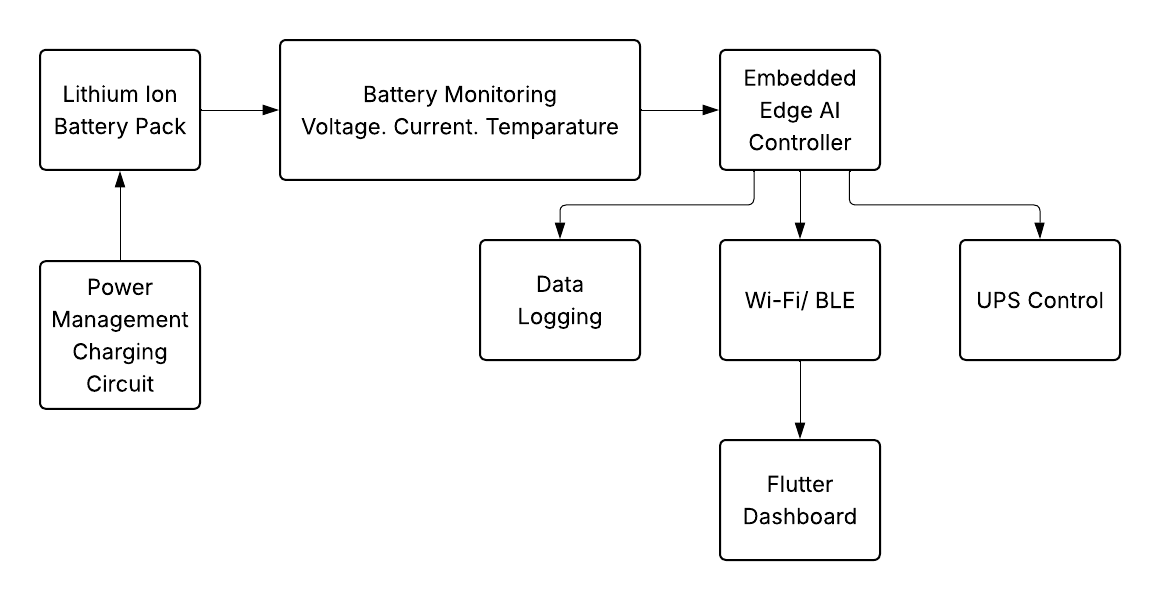
\includegraphics[width=\textwidth,height=0.90 \textheight,keepaspectratio]{prism-uploads/Blank diagram (28).png}
    \caption{Block Diagram of Edge AI Smart Battery Management System with Intelligent UPS}
  \end{figure}
\end{frame}

\begin{frame}{Prepared Battery Dataset Sample}
  \setbeamertemplate{caption}[numbered]
  \begin{figure}
    \centering
    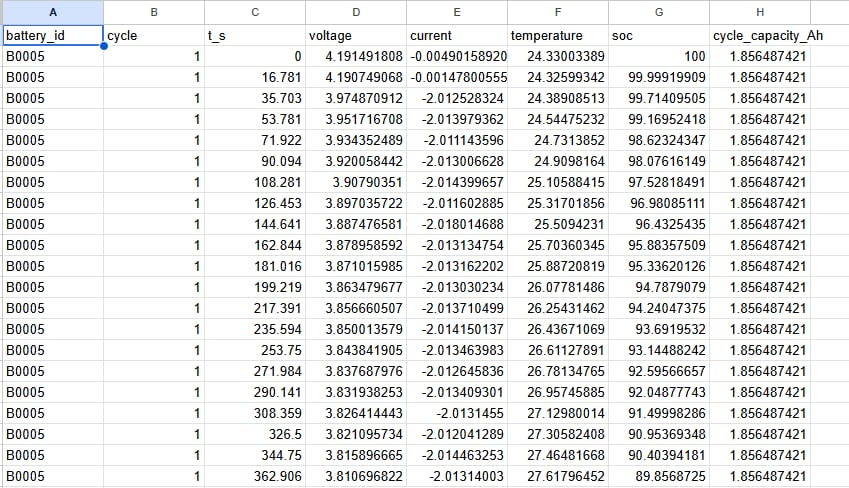
\includegraphics[width=\textwidth,height=0.72\textheight,keepaspectratio]{prism-uploads/image_14.png}
    \caption{Representative rows from the prepared battery dataset used for SOC and SOH model training.}
  \end{figure}
\end{frame}

\section{Design Formulation and Progress}
\begin{frame}{Design Formulation and Progress}
  \begin{columns}[T,onlytextwidth]
    \begin{column}{0.48\textwidth}
      \begin{block}{Hardware}
        \footnotesize
        \begin{itemize}
          \setlength{\itemsep}{3pt}
          \item 3S Li-ion pack: 9--12.6 V; cell taps sensed on GPIO 4, 5, and 6.
          \item INA226 measures current, bus voltage, and power over I$^2$C (GPIO 8/9).
          \item Three 10 k$\Omega$ NTCs monitor cell temperatures on GPIO 1, 2, and 7.
          \item ESP32-S3 provides local processing, Wi-Fi, and USB debugging.
        \end{itemize}
      \end{block}
    \end{column}
    \hfill
    \begin{column}{0.48\textwidth}
      \begin{block}{Software}
        \footnotesize
        \begin{itemize}
          \setlength{\itemsep}{3pt}
          \item 1 Hz loop samples sensors, calibrates readings, estimates SOC, and reports data.
          \item Serial commands support logging, cycle tracking, and CSV output.
          \item Monitoring includes cell imbalance and load activity detection.
          \item Flutter app presents live status, analytics, predictions, alerts, and settings.
        \end{itemize}
      \end{block}
    \end{column}
  \end{columns}
\end{frame}

\begin{frame}{Design Formulation and Progress (Contd.)}
  \footnotesize
  \begin{columns}[T,onlytextwidth]
    \begin{column}{0.48\textwidth}
      \begin{itemize}
        \setlength{\itemsep}{9pt}
        \item \textbf{Hardware and firmware — Complete.} ESP32-S3 prototype integrates three cell taps, INA226 current sensing, and three NTCs. Firmware samples and calibrates readings for local monitoring.
        \item \textbf{ADC calibration — In progress.} Quadratic fits improve voltage accuracy; Tap 3 still needs recalibration.
        \item \textbf{NASA dataset Preprocessing — Complete.}    \\  Cycling records are cleaned and organized as time series with voltage, current, temperature, SOC, and capacity fields.
      \end{itemize}
    \end{column}
    \hfill
    \begin{column}{0.48\textwidth}
      \begin{itemize}
        \setlength{\itemsep}{9pt}
        \item \textbf{SOC models — Complete.} \\ RF, MLP, and LSTM were compared with Coulomb counting using battery-level splits; Fine-Tuned MLP preferred for edge-deployment.
        \item \textbf{SOH/RUL models — In progress.} Aging- and capacity-based estimators are under development; evaluation and optimization remain before embedded deployment.
        \item \textbf{Flutter app — Complete.} \\ The 11-screen app displays battery status, telemetry, analytics, predictions, alerts, and settings.
      \end{itemize}
    \end{column}
  \end{columns}
\end{frame}




\section{Results and Discussion}
\begin{frame}{Results and Discussion}
  \footnotesize
  \renewcommand{\arraystretch}{1.15}
  {\centering
  \begin{tabularx}{0.86\textwidth}{|Y|c|c|c|}
    \hline
    \multicolumn{1}{|c|}{\parbox{0.30\textwidth}{\centering\textbf{Model}}} &
    \textbf{MAE (\%)} & \textbf{RMSE (\%)} & \textbf{$R^2$} \\ \hline
    Coulomb counting & 4.266 & 7.540 & 0.9273 \\ \hline
    Random Forest & 3.587 & 5.152 & 0.9661 \\ \hline
    XGBoost & 3.964 & 5.401 & 0.9627 \\ \hline
    Simplified MLP / DNN & 7.591 & 9.693 & 0.8799 \\ \hline
    \textbf{Fine-tuned MLP / DNN} & \textbf{4.647} & \textbf{6.274} & \textbf{0.9497} \\ \hline
    LSTM & 7.070 & 9.275 & 0.8900 \\ \hline
  \end{tabularx}\par}
  \vspace{4pt}
  {\centering\textbf{Table 5. SOC Model Performance Comparison}\par}
  \vspace{3pt}

  \begin{block}{Key Finding}
    \textbf{The fine-tuned MLP} is preferred for edge deployment because its lightweight design, low complexity, and small footprint suit microcontrollers. It achieves MAE of 4.647\%, RMSE of 6.274\%, and $R^2$ of 0.9497.
  \end{block}
  \vspace{-3pt}
\end{frame}



\begin{frame}{SOC Model Comparison - MAE per Battery}
  \setbeamertemplate{caption}[numbered]
  \begin{figure}
    \centering
    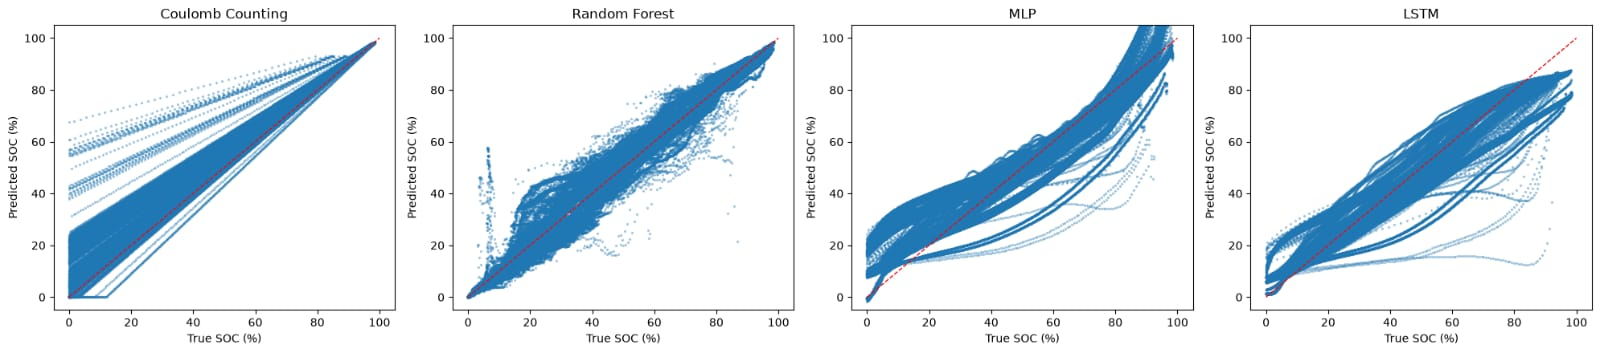
\includegraphics[width=\textwidth,height=0.62\textheight,keepaspectratio]{prism-uploads/image_6.png}
    \par\vspace{2pt}
    \begin{minipage}{0.24\textwidth}\centering\scriptsize (a) Coulomb counting\end{minipage}\hfill
    \begin{minipage}{0.24\textwidth}\centering\scriptsize (b) Random Forest\end{minipage}\hfill
    \begin{minipage}{0.24\textwidth}\centering\scriptsize (c) MLP\end{minipage}\hfill
    \begin{minipage}{0.24\textwidth}\centering\scriptsize (d) LSTM\end{minipage}
    \caption{Actual versus predicted State of Charge (SOC) for four estimation methods.}
  \end{figure}
\end{frame}

\begin{frame}{Fine-Tuned MLP: Actual vs. Predicted SOC}
  \setbeamertemplate{caption}[numbered]
  \begin{figure}
    \centering
    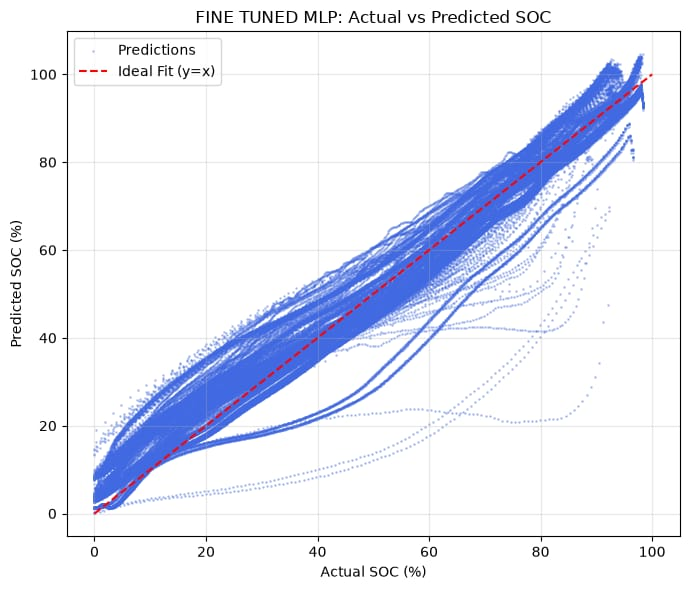
\includegraphics[width=\textwidth,height=0.72\textheight,keepaspectratio]{prism-uploads/image_11.png}
    \caption{Actual versus predicted SOC for the fine-tuned MLP model.}
  \end{figure}
\end{frame}

\begin{frame}{SOH Estimation: Actual vs. Predicted}
  \setbeamertemplate{caption}[numbered]
  \begin{figure}
    \centering
    \begin{minipage}{0.48\textwidth}
      \centering
      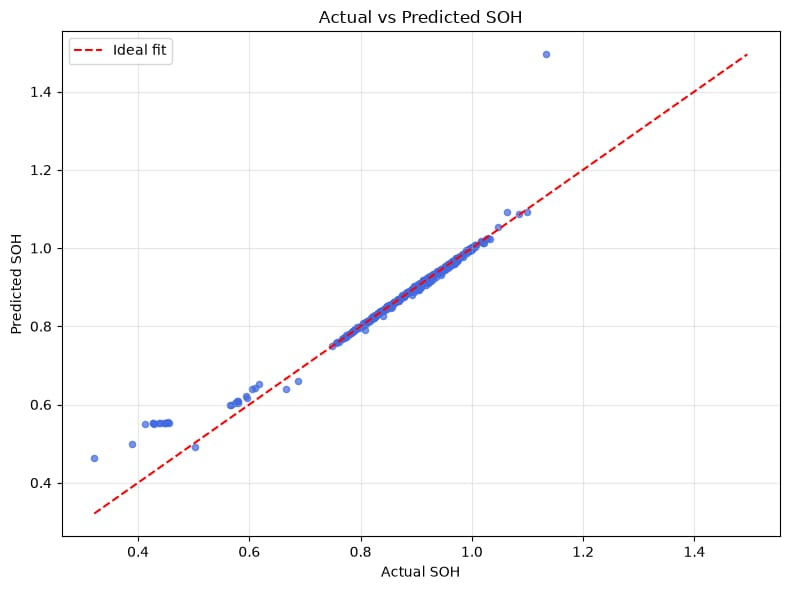
\includegraphics[width=\linewidth,height=0.62\textheight,keepaspectratio]{prism-uploads/image_12.png}
      \par\small (a) XGBoost based SOH estimation
    \end{minipage}\hfill
    \begin{minipage}{0.48\textwidth}
      \centering
      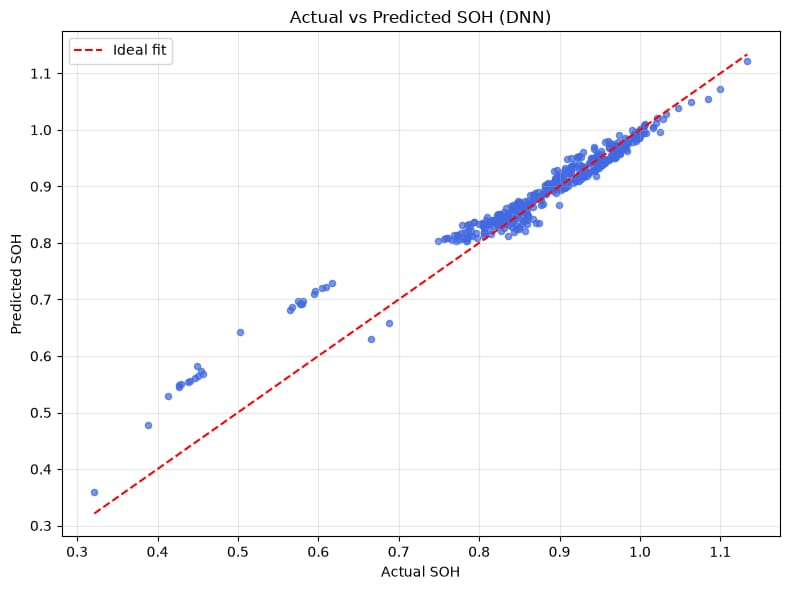
\includegraphics[width=\linewidth,height=0.62\textheight,keepaspectratio]{prism-uploads/image_13.png}
      \par\small (b) DNN-based SOH estimation
    \end{minipage}
    \caption{Actual versus Predicted SOH; dashed lines indicate ideal fit.}
  \end{figure}
\end{frame}

\begin{frame}{SOH Estimation: Model Comparison}
  \footnotesize
  \renewcommand{\arraystretch}{1.2}
  {\centering
  \begin{tabularx}{0.86\textwidth}{|Y|c|c|c|}
    \hline
    \multicolumn{1}{|c|}{\textbf{Model}} &
    \textbf{MAE (\%)} & \textbf{RMSE (\%)} & \textbf{$R^2$} \\ \hline
    XGBoost & 0.0072 & 0.0270 & 0.9494 \\ \hline
    \textbf{DNN} & \textbf{0.0194} & \textbf{0.0320} & \textbf{0.9287} \\ \hline
  \end{tabularx}\par}
  \par\vspace{3pt}{\centering\textbf{Table 6. SOH Model Performance Comparison}\par}
  \vspace{5pt}
  \begin{block}{Key Finding}
    DNN is preferred for edge deployment because compared to XGBoost it is lightweight , less complex, and have small footprint suit microcontrollers. It achieves MAE of 0.0194\%, RMSE of 0.0320\%, and $R^2$ of 0.9287.
  \end{block}
\end{frame}

\begin{frame}{Discussion: Limitations and Deployment Challenges}
  \small
  \begin{itemize}
    \setlength{\itemsep}{6pt}
    \item \textbf{Dataset Limitations}: NASA data contains four discrete current levels ($0$, $-1$, $-2$, and $-4$~A), limiting real-world variable-load representation.
    \item \textbf{Voltage--SOC Dependence}: Hysteresis (0.3--0.5~V), temperature, and aging affect the voltage--SOC relationship.
    \item \textbf{Model Generalization}: Test batteries B0038 and B0054 showed systematic prediction errors, indicating possible limitations across battery units.
    \item \textbf{Limitations of Conventional SOC Estimation}: Coulomb counting suffers from cumulative integration errors and initial SOC uncertainty, motivating ML-based estimation. However, ML accuracy depends on reference-label quality.
    \item \textbf{Edge Deployment and Validation}: The fine-tuned MLP (SOC) and DNN (SOH) were selected for deployment feasibility. ESP32-S3 inference and validation under variable loads and temperatures remain pending.
  \end{itemize}
\end{frame}
\begin{frame}{Hardware Setup}
  \setbeamertemplate{caption}[numbered]
  \begin{figure}
    \centering
    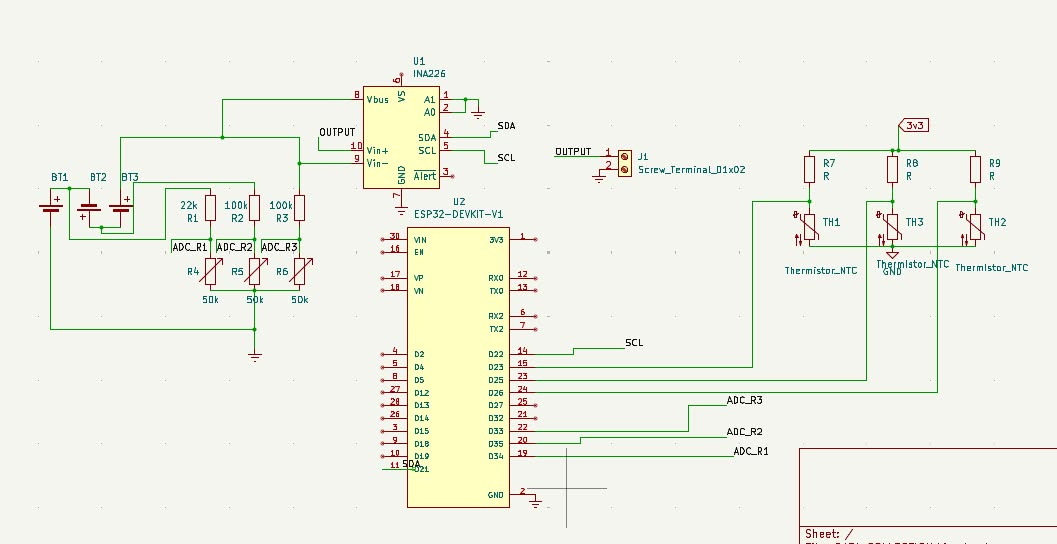
\includegraphics[width=\textwidth,height=0.70\textheight,keepaspectratio]{prism-uploads/image_17.png}
    \caption{Hardware setup of the Edge AI Smart Battery Management System.}
  \end{figure}
\end{frame}

\begin{frame}{System Implementation and Functional Features}
  \footnotesize
  \begin{columns}[T,onlytextwidth]
    \begin{column}{0.47\textwidth}
      \begin{block}{ESP32-S3 Firmware Capabilities}
        \begin{itemize}
          \setlength{\itemsep}{3pt}
          \item Three-cell voltage monitoring with quadratic calibration.
          \item Load-current measurement using INA226.
          \item Temperature sensing with three NTC thermistors.
          \item NASA-compatible CSV output and serial command interface.
          \item Cycle tracking with capacity integration.
          \item Cell-imbalance detection.
          \item SoC estimation using a linear method.
        \end{itemize}
      \end{block}
    \end{column}
    \begin{column}{0.47\textwidth}
      \begin{block}{Flutter App Features}
        \begin{itemize}
          \setlength{\itemsep}{3pt}
          \item Real-time dashboard with circular SoC indicator.
          \item Historical voltage, current, temperature, SoC, SOH, and power analytics.
          \item AI prediction screen with degradation forecast.
          \item Battery details with cell-level monitoring.
          \item Severity-level alerts and device-management settings.
          \item Dark and light themes.
          \item OTA update interface (UI ready).
        \end{itemize}
      \end{block}
    \end{column}
  \end{columns}
\end{frame}

\begin{frame}{Prototype Performance Metrics}
  \scriptsize
  \renewcommand{\arraystretch}{1.5}
  \begin{tabularx}{\textwidth}{|L{0.22\textwidth}|L{0.18\textwidth}|Y|}
    \hline
    \multicolumn{1}{|c|}{\textbf{Metric}} & \multicolumn{1}{c|}{\textbf{Target}} & \multicolumn{1}{c|}{\textbf{Achieved}} \\ \hline
    SOC MAE & $<5\%$ & 3.59\% \\ \hline
    ADC Accuracy & $<50$ mV & 31.5 mV (Tap 1); 56 mV (Tap 2) \\ \hline
    Voltage Resolution & 12-bit & 12-bit \\ \hline
    Current Sensing & $\pm0.8$ A & $\pm0.8$ A \\ \hline
    Temperature Sensing & 3 cells & 3 cells \\ \hline
    Mobile Screens & 8+ & 11 \\ \hline
  \end{tabularx}
  \par\vspace{2pt}{\centering\textbf{Table 7. Hardware and Dashboard Performance Metrics}\par}
  \vspace{7pt}

  \textbf{Conclusion}\par
  \vspace{2pt}
  {\footnotesize The prototype combines embedded sensing, Edge AI, and mobile visualization. UPS/OTA integration and end-to-end validation remain in progress toward reliable deployment.}
\end{frame}

 

\section{Individual Contributions and Teamwork}
\begin{frame}{Individual Contributions \& Teamwork}
  \scriptsize
  \renewcommand{\arraystretch}{1.2}
  \begin{tabularx}{\textwidth}{|L{0.22\textwidth}|Y|}
    \hline
    \multicolumn{1}{|c|}{\textbf{Member}} & \multicolumn{1}{c|}{\textbf{Responsibilities}} \\ \hline
    Harikesh OP & Embedded firmware, ML models, and hardware integration. \\ \hline
    Amaya Promod PV & Literature review, NASA dataset study, and data augmentation. \\ \hline
    Nandana Jayachandran & Dataset analysis and data augmentation. \\ \hline
    Pooja K & Documentation and supporting tasks. \\ \hline
  \end{tabularx}
  \par\vspace{2pt}{\centering\textbf{Table 6. Team Member Contributions}\par}
  \vspace{4pt}

  \begin{columns}[T,onlytextwidth]
    \begin{column}{0.48\textwidth}
      \begin{block}{Teamwork \& Collaboration}
        \scriptsize
        \begin{itemize}
          \setlength{\itemsep}{2pt}
          \item Regular progress meetings and code reviews.
          \item Collaborative debugging and knowledge sharing.
          \item Coordinated hardware--software integration.
        \end{itemize}
      \end{block}
    \end{column}
    \begin{column}{0.48\textwidth}
      \begin{block}{Tools \& Technologies}
        \scriptsize
        \textbf{Embedded:} C++, Arduino, PlatformIO, ESP32/S3\par
        \textbf{ML/Data:} Python, pandas, scikit-learn, TensorFlow/Keras, NumPy\par
        \textbf{Mobile:} Flutter, Dart, Provider, fl\_chart\par
        \textbf{Hardware:} INA226, NTC thermistors, voltage dividers\par
        \textbf{Tools:} Git, Jupyter, VS Code, Arduino IDE
      \end{block}
    \end{column}
  \end{columns}
\end{frame}



\section{Work Plan}
\begin{frame}{Work Plan}
  \footnotesize
  \begin{itemize}
    \setlength{\itemsep}{6pt}
    \item \textbf{Phase 1 -- Research \& Design (Weeks 1--4, complete):} Literature review, NASA dataset study, system architecture, and hardware selection.
    \item \textbf{Phase 2 -- Data Preparation (Weeks 5--8, complete):} Dataset extraction, cleaning, preprocessing, analysis, and train/test split.
    \item \textbf{Phase 3 -- ML Development (Weeks 9--12, complete):} Coulomb counting baseline; RF, MLP, and LSTM training, evaluation, and comparison.
    \item \textbf{Phase 4 -- Hardware (Weeks 13--16, complete):} ESP32/S3 firmware, ADC calibration, INA226, NTC sensing, and NASA data mode.
    \item \textbf{Phase 5 -- Mobile App (Weeks 17--20, complete):} Flutter architecture, dashboard, analytics, AI predictions, settings, and themes.
    \item \textbf{Phase 6 -- Integration \& Testing (Weeks 21--24, in progress):} Wi-Fi, SD logging, OTA, system tests, fixes, and optimization.
  \end{itemize}
\end{frame}

\begin{frame}{Project Schedule \& Progress (Gantt Chart)}
  \centering
  \resizebox{0.96\textwidth}{!}{%
  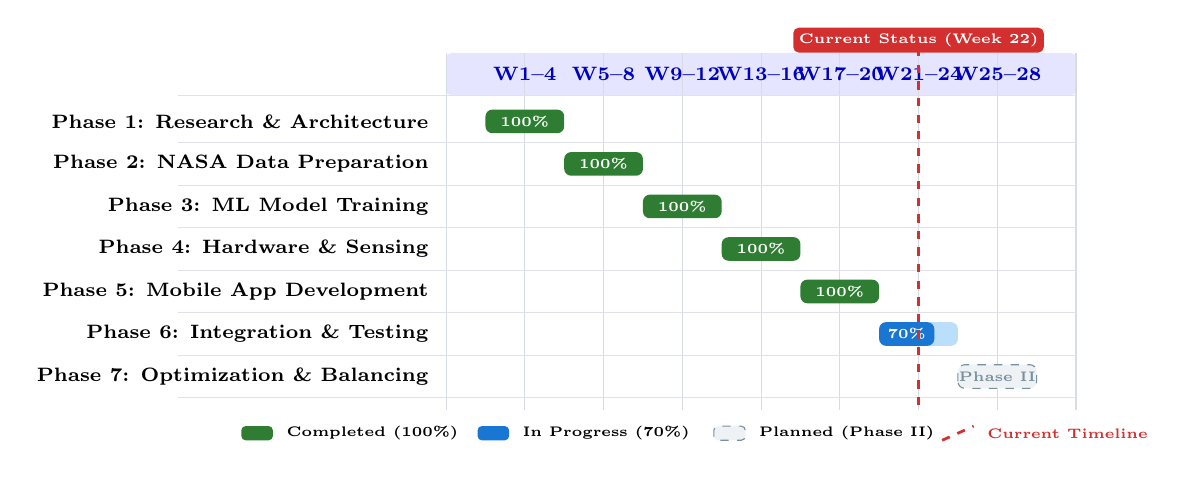
\begin{tikzpicture}[x=1cm,y=0.60cm]
    % Color definitions
    \definecolor{cComplete}{RGB}{46, 125, 50}
    \definecolor{cProgress}{RGB}{25, 118, 210}
    \definecolor{cProgressLight}{RGB}{187, 222, 251}
    \definecolor{cPlanned}{RGB}{120, 144, 156}
    \definecolor{cPlannedLight}{RGB}{238, 242, 245}
    \definecolor{cCurrent}{RGB}{211, 47, 47}
    \definecolor{gridLine}{RGB}{215, 220, 228}

    % Header background
    \fill[blue!10, rounded corners=2pt] (3.6, 0.45) rectangle (11.6, -0.45);

    % Column headers & vertical gridlines
    \foreach \x/\label in {
      4.6/{W1--4},
      5.6/{W5--8},
      6.6/{W9--12},
      7.6/{W13--16},
      8.6/{W17--20},
      9.6/{W21--24},
      10.6/{W25--28}
    } {
      \draw[gridLine, line width=0.4pt] (\x, 0.45) -- (\x, -7.1);
      \node[font=\bfseries\scriptsize, text=blue!75!black] at (\x, 0) {\label};
    }
    \draw[gridLine, line width=0.4pt] (3.6, 0.45) -- (3.6, -7.1);
    \draw[gridLine, line width=0.4pt] (11.6, 0.45) -- (11.6, -7.1);

    % Row 1
    \node[anchor=east, font=\scriptsize\bfseries] at (3.5, -1) {Phase 1: Research \& Architecture};
    \fill[cComplete, rounded corners=2.5pt] (4.1, -1.25) rectangle (5.1, -0.75);
    \node[font=\tiny\bfseries, text=white] at (4.6, -1) {100\%};

    % Row 2
    \node[anchor=east, font=\scriptsize\bfseries] at (3.5, -1.9) {Phase 2: NASA Data Preparation};
    \fill[cComplete, rounded corners=2.5pt] (5.1, -2.15) rectangle (6.1, -1.65);
    \node[font=\tiny\bfseries, text=white] at (5.6, -1.9) {100\%};

    % Row 3
    \node[anchor=east, font=\scriptsize\bfseries] at (3.5, -2.8) {Phase 3: ML Model Training};
    \fill[cComplete, rounded corners=2.5pt] (6.1, -3.05) rectangle (7.1, -2.55);
    \node[font=\tiny\bfseries, text=white] at (6.6, -2.8) {100\%};

    % Row 4
    \node[anchor=east, font=\scriptsize\bfseries] at (3.5, -3.7) {Phase 4: Hardware \& Sensing};
    \fill[cComplete, rounded corners=2.5pt] (7.1, -3.95) rectangle (8.1, -3.45);
    \node[font=\tiny\bfseries, text=white] at (7.6, -3.7) {100\%};

    % Row 5
    \node[anchor=east, font=\scriptsize\bfseries] at (3.5, -4.6) {Phase 5: Mobile App Development};
    \fill[cComplete, rounded corners=2.5pt] (8.1, -4.85) rectangle (9.1, -4.35);
    \node[font=\tiny\bfseries, text=white] at (8.6, -4.6) {100\%};

    % Row 6
    \node[anchor=east, font=\scriptsize\bfseries] at (3.5, -5.5) {Phase 6: Integration \& Testing};
    \fill[cProgressLight, rounded corners=2.5pt] (9.1, -5.75) rectangle (10.1, -5.25);
    \fill[cProgress, rounded corners=2.5pt] (9.1, -5.75) rectangle (9.8, -5.25);
    \node[font=\tiny\bfseries, text=white] at (9.45, -5.5) {70\%};

    % Row 7
    \node[anchor=east, font=\scriptsize\bfseries] at (3.5, -6.4) {Phase 7: Optimization \& Balancing};
    \draw[cPlanned, dashed, fill=cPlannedLight, rounded corners=2.5pt] (10.1, -6.65) rectangle (11.1, -6.15);
    \node[font=\tiny\bfseries, text=cPlanned] at (10.6, -6.4) {Phase II};

    % Horizontal row divider lines
    \foreach \y in {-0.45, -1.45, -2.35, -3.25, -4.15, -5.05, -5.95, -6.85} {
      \draw[gridLine!80, line width=0.3pt] (0.2, \y) -- (11.6, \y);
    }

    % Milestone line
    \draw[cCurrent, dashed, line width=1.1pt] (9.6, 0.55) -- (9.6, -7.1);
    \node[fill=cCurrent, text=white, font=\tiny\bfseries, rounded corners=2pt, inner sep=2pt] at (9.6, 0.72) {Current Status (Week 22)};

    % Legend
    \begin{scope}[shift={(1.0, -7.6)}]
      \fill[cComplete, rounded corners=1.5pt] (0, -0.15) rectangle (0.4, 0.15);
      \node[anchor=west, font=\tiny\bfseries] at (0.45, 0) {Completed (100\%)};

      \fill[cProgress, rounded corners=1.5pt] (3.0, -0.15) rectangle (3.4, 0.15);
      \node[anchor=west, font=\tiny\bfseries] at (3.45, 0) {In Progress (70\%)};

      \draw[cPlanned, dashed, fill=cPlannedLight, rounded corners=1.5pt] (6.0, -0.15) rectangle (6.4, 0.15);
      \node[anchor=west, font=\tiny\bfseries] at (6.45, 0) {Planned (Phase II)};

      \draw[cCurrent, dashed, line width=1pt] (8.9, -0.15) -- (9.3, 0.15);
      \node[anchor=west, font=\tiny\bfseries, text=cCurrent] at (9.35, 0) {Current Timeline};
    \end{scope}
  \end{tikzpicture}
  }
  \vspace{4pt}
  \begin{block}{Progress Summary}
    \scriptsize
    Phases 1--5 are 100\% complete. Phase 6 (System Integration \& Validation) is actively underway at 70\% completion, targeting end-to-end telemetry, UPS changeover, and field testing prior to Phase II deployment.
  \end{block}
\end{frame}

\section{Project Budget}
\begin{frame}[t]{Project Budget \& Component Cost Breakdown}
  \centering
  \fontsize{6.5pt}{7.6pt}\selectfont
  \renewcommand{\arraystretch}{0.95}
  \setlength{\tabcolsep}{2.5pt}
  \definecolor{budgethead}{RGB}{230,235,245}

  \begin{tabularx}{\textwidth}{|c|X|p{0.27\textwidth}|c|r|r|c|}
    \hline
    \rowcolor{budgethead}
    \textbf{No.} & \textbf{Component / Module} & \textbf{Specification / Purpose} & \textbf{Qty} & \textbf{Rate (Rs.)} & \textbf{Cost (Rs.)} & \textbf{Status} \\ \hline
    1 & ESP32-S3 DevKit-N16R8 & Dual Xtensa LX7, 8MB PSRAM, Wi-Fi & 1 & 650 & 650 & \textcolor{green!50!black}{\textbf{Procured}} \\ \hline
    2 & INA226 Sensor Module & $I^2$C Bi-dir Current/Bus Monitor ($0.1\,\Omega$) & 1 & 280 & 280 & \textcolor{green!50!black}{\textbf{Procured}} \\ \hline
    3 & 3S Li-ion Battery Pack & 18650 Cells (11.1\,V nominal, 2600\,mAh) & 3 & 250 & 750 & \textcolor{green!50!black}{\textbf{Procured}} \\ \hline
    4 & NTC Thermistors ($10\,\text{k}\Omega$) & Cell temperature monitoring ($B=3950$) & 3 & 30 & 90 & \textcolor{green!50!black}{\textbf{Procured}} \\ \hline
    5 & Voltage Divider Resistors & Carbon-film resistors \& trimpots / caps & 1 set & 80 & 80 & \textcolor{green!50!black}{\textbf{Procured}} \\ \hline
    6 & UPS Switching Circuit & Auto-cutover relay, MOSFETs \& buck module & 1 & 350 & 350 & \textcolor{orange!85!black}{\textbf{Not Procured}} \\ \hline
    7 & MicroSD Logging Module & SPI interface with 16\,GB Class 10 card & 1 & 260 & 260 & \textcolor{orange!85!black}{\textbf{Not Procured}} \\ \hline
    8 & Prototyping \& Packaging & Perfboard, terminal blocks, wiring harness & 1 set & 190 & 190 & \textcolor{green!50!black}{\textbf{Procured}} \\ \hline
    \rowcolor{blue!12}
    \multicolumn{5}{|r|}{\textbf{Total Budget (Procured: Rs.~2,040 \;|\; Pending: Rs.~610):}} & \textbf{Rs.~2,650} & \textbf{Within Budget} \\ \hline
  \end{tabularx}
  \par\vspace{1pt}

  \begin{columns}[T,onlytextwidth]
    \begin{column}{0.48\textwidth}
      \begin{block}{Cost Effectiveness}
        \fontsize{6pt}{7.2pt}\selectfont
        \begin{itemize}
          \setlength{\itemsep}{1pt}
          \item \textbf{Commercial Smart BMS:} Typically Rs.~12,000--25,000 (\$150--\$300).
          \item \textbf{Proposed Prototype:} Full build within \textbf{Rs.~2,650} (\$32); \textbf{Rs.~2,040} utilized for active hardware to date.
        \end{itemize}
      \end{block}
    \end{column}
    \begin{column}{0.48\textwidth}
      \begin{block}{PO11 Alignment (Finance \& Management)}
        \fontsize{6pt}{7.2pt}\selectfont
        \begin{itemize}
          \setlength{\itemsep}{1pt}
          \item Quadratic ADC calibration compensates for standard carbon resistor tolerances without costly AFEs.
          \item Phased procurement: UPS and SD logger scheduled for final integration milestone.
        \end{itemize}
      \end{block}
    \end{column}
  \end{columns}
\end{frame}

\section{Future Activities}
\begin{frame}{Future Activities}
  \small
  \begin{itemize}
    \item ADC Calibration improvement
    \item Wi-Fi Integration
    \item OTA Firmware Updates 
    \item SOH and RUL Models
    \item Real hardware data collection
    \item Model Optimization for Edge deployment
    \item Cascaded SOC--SOH Architecture
    \item Cell balancing Implementation
    \item Advanced Protection Features
    \item Multi-pack Support
    \item {Production Readiness}
  \end{itemize}
\end{frame}

\section{Project Summary}
\begin{frame}{Project Summary}
  \footnotesize
  \textbf{Objective}\par
  \vspace{2pt}
  Develop an intelligent BMS that protects lithium-ion batteries, predicts battery health using Edge AI, and aims to provide uninterrupted power through an integrated UPS.
  \vspace{7pt}
 
  \begin{columns}[T,onlytextwidth]
    \begin{column}{0.55\textwidth}
      \begin{block}{Key Achievements}
        \begin{itemize}
          \setlength{\itemsep}{3pt}
            \item Hardware Prototype
            \item Machine Learning Models
            \item Data Pipeline
            \item Mobile Application
            \item Firmware features
        \end{itemize}
      \end{block}
    \end{column}
    \begin{column}{0.41\textwidth}
      \begin{block}{Novel Contributions}
        \begin{itemize}
          \setlength{\itemsep}{4pt}
          \item End-to-end system
          \item Comparative ML study
          \item Data Quality Improvements
          \item Real Hardware Implementation
        \end{itemize}
      \end{block}
    \end{column}
  \end{columns}

  \vspace{8pt}
  \textbf{Conclusion}\par
      \vspace{3pt}
      The prototype combines embedded sensing, Edge AI, and mobile visualization. UPS/OTA integration and end-to-end validation remain in progress toward reliable deployment.
\end{frame}
 



\section{References}
\begin{frame}[t]{References}
  \footnotesize
  \begin{itemize}
    \setlength{\itemsep}{4pt}
    \item[{[1]}] R. Xiong, J. Cao, Q. Yu, H. He, and F. Sun, ``Critical Review on the Battery State of Charge Estimation Methods for Electric Vehicles,'' \textit{IEEE Access}, vol. 6, pp. 1832--1843, 2018, doi: 10.1109/ACCESS.2017.2780258.
    \item[{[2]}] Chemali et al., ``Long Short-Term Memory Networks for Accurate State-of-Charge Estimation of Li-ion Batteries,'' \textit{IEEE Transactions on Industrial Electronics}, vol. 65, no. 8, pp. 6730--6739, Aug. 2018, doi: 10.1109/TIE.2017.2787586.
    \item[{[3]}] Crocioni et al., ``Li-Ion Batteries Parameter Estimation With Tiny Neural Networks Embedded on Intelligent IoT Microcontrollers,'' \textit{IEEE Access}, vol. 8, pp. 122135--122146, 2020, doi: 10.1109/ACCESS.2020.3007046.
    \item[{[4]}] P. Venugopal, S. S. Shankar, C. P. Jebakumar, R. Agarwal, H. H. Alhelou, S. S. Reka, and M. E. H. Golshan, ``Analysis of Optimal Machine Learning Approach for Battery Life Estimation of Li-Ion Cell,'' \textit{IEEE Access}, vol. 9, pp. 159616--159626, 2021, doi: 10.1109/ACCESS.2021.3130994.
  \end{itemize}
\end{frame}

\begin{frame}[t]{References}
  \footnotesize
  \begin{itemize}
    \setlength{\itemsep}{4pt}
    \item[{[5]}] H. M. Hussein, M. Esoofally, A. Donekal, S. M. S. H. Rafin, and O. Mohammed, ``Comparative Study-Based Data-Driven Models for Lithium-Ion Battery State-of-Charge Estimation,'' \textit{Batteries}, vol. 10, no. 3, Art. no. 89, 2024, doi: 10.3390/batteries10030089.
    \item[{[6]}] S. Giazitzis, M. Sakwa, S. Leva, E. Ogliari, S. Badha, and F. Rosetti, ``A Case Study of a Tiny Machine Learning Application for Battery State-of-Charge Estimation,'' \textit{Electronics}, vol. 13, no. 10, Art. no. 1964, 2024, doi: 10.3390/electronics13101964.
    \item[{[7]}] P. Li, X. Wu, R. Grosu, J. Hou, M. Ilolov, and S. Xiang, ``Applying Neural Network to Health Estimation and Lifetime Prediction of Lithium-Ion Batteries,'' \textit{IEEE Transactions on Transportation Electrification}, vol. 11, no. 1, pp. 4224--4248, 2025, doi: 10.1109/TTE.2024.3457621.
    \item[{[8]}] G. Giazitzis, J. Ferrari, A. J. Woss, S. Badha, F. Rosetti, and E. Ogliari, ``Embedded Strategy for Battery Module States Estimation Using Tiny Machine Learning Models,'' \textit{Journal of Energy Storage}, vol. 152, Art. no. 120673, 2026, doi: 10.1016/j.est.2026.120673.
  \end{itemize}
\end{frame}

\section{Appendix A: NBA Accreditation Criteria}
\definecolor{mappingheader}{RGB}{239,237,221}

\begin{frame}{Appendix A: NBA Accreditation Criteria}
  \footnotesize
  \centering
  \renewcommand{\arraystretch}{1.15}
  \setlength{\tabcolsep}{2pt}
  \textbf{Table A.1: Student Capstone Projects with PO, PSO and Sustainability Mapping}\par
  \vspace{5pt}
  \begin{tabularx}{0.98\textwidth}{|p{0.045\textwidth}|p{0.22\textwidth}|p{0.11\textwidth}|p{0.12\textwidth}|X|p{0.10\textwidth}|}
    \hline
    \rowcolor{mappingheader}
    \multicolumn{1}{|c|}{\parbox{0.045\textwidth}{\centering\scriptsize\textbf{Sl. No.}}} &
    \multicolumn{1}{c|}{\parbox{0.22\textwidth}{\centering\textbf{Project Title}}} &
    \multicolumn{1}{c|}{\parbox{0.11\textwidth}{\centering\textbf{Guide}}} &
    \multicolumn{1}{c|}{\parbox{0.12\textwidth}{\centering\textbf{Type}}} &
    \multicolumn{1}{c|}{\parbox{0.30\textwidth}{\centering\textbf{Domain}}} &
    \multicolumn{1}{c|}{\parbox{0.10\textwidth}{\centering\textbf{SDGs}}} \\ \hline
    1 & Edge AI Smart Battery Management System with Intelligent UPS & Dr. Sajith K & Product-oriented & Embedded Systems, Edge AI, IoT, and Mobile Application Development & SDG 7, 9, 11 \\ \hline
  \end{tabularx}
  \par\vspace{8pt}
  \renewcommand{\arraystretch}{1.15}
  \setlength{\tabcolsep}{1.5pt}
 
  \vspace{3pt}
  \begin{tabularx}{0.98\textwidth}{|>{\centering\arraybackslash}p{0.14\textwidth}|>{\centering\arraybackslash}p{0.08\textwidth}|>{\centering\arraybackslash}p{0.09\textwidth}|>{\centering\arraybackslash}p{0.06\textwidth}|>{\centering\arraybackslash}p{0.17\textwidth}|>{\centering\arraybackslash}p{0.15\textwidth}|>{\raggedright\arraybackslash}X|}
    \hline
    \rowcolor{mappingheader}
    \textbf{Environment} & \textbf{Safety} & \textbf{Ethics} & \textbf{Cost} & \textbf{Standards} & \textbf{POs \& PSOs} & \textbf{POs \& PSOs Justification} \\ \hline
    Low to Moderate impact & Low risk & Low concern & Low & IEEE 802.11 (Wi-Fi), IEC 62660-1, and IEEE 1725 & PO1--PO5, PO7, PO9--PO12; PSO1--PSO3 & Integrates embedded systems and Edge AI for intelligent battery monitoring, model evaluation, and sustainable battery usage. \\ \hline
  \end{tabularx}
\end{frame}

\begin{frame}{Appendix A: NBA Accreditation Criteria (Contd.)}
  \scriptsize
  \centering
  \renewcommand{\arraystretch}{1.0}
  \setlength{\tabcolsep}{2pt}
  \textbf{PO Mapping Justification}\par
  \vspace{2pt}
  \begin{tabularx}{0.96\textwidth}{|p{0.12\textwidth}|X|}
    \hline
    \rowcolor{mappingheader}\multicolumn{1}{|c|}{\textbf{PO}} & \multicolumn{1}{c|}{\textbf{Justification}} \\ \hline
    PO1 & Applied engineering and mathematics to BMS design, quadratic ADC calibration, voltage dividers, and NTC sensing. \\ \hline
    PO2 & Analyzed conventional BMS limits, NASA data-quality issues, and out-of-distribution battery behavior. \\ \hline
    PO3 & Designed system architecture and developed ESP32-S3 firmware, ML estimators, and a Flutter app. \\ \hline
    PO4 & Conducted NASA EDA, hysteresis and aging analysis, and systematic model comparisons. \\ \hline
    PO5 & Used Python, scikit-learn, TensorFlow, PlatformIO, Flutter, and Git. \\ \hline
    PO7 & Predictive maintenance supports longer battery life, less waste, and efficient energy use. \\ \hline
    PO9 & Led firmware development; collaborated on ML and integration through meetings and reviews. \\ \hline
    PO10 & Prepared project documentation, technical reports, and presentations. \\ \hline
    PO11 & Managed phased milestones, budget-conscious components, risks, and future resources. \\ \hline
    PO12 & Learned Flutter, TensorFlow, and ESP32-S3 and iteratively improved the system using research findings. \\ \hline
  \end{tabularx}
  \par\vspace{4pt}
  \textbf{PSO Mapping Justification}\par
  \vspace{1pt}
  \begin{tabularx}{0.96\textwidth}{|p{0.12\textwidth}|X|}
    \hline
    \rowcolor{mappingheader}\multicolumn{1}{|c|}{\textbf{PSO}} & \multicolumn{1}{c|}{\textbf{Justification}} \\ \hline
    PSO1 & Hands-on competence in electronic circuits and embedded systems. \\ \hline
    PSO2 & Proficiency in ML programming and software tools. \\ \hline
    PSO3 & Application of instrumentation and monitoring techniques for battery management. \\ \hline
  \end{tabularx}
\end{frame}

\begin{frame}{Appendix A: NBA Accreditation Criteria (Contd.)}
  \scriptsize
  \centering
  \renewcommand{\arraystretch}{1.1}
  \setlength{\tabcolsep}{4pt}
  \textbf{SDG Mapping Justification}\par
  \vspace{3pt}
  \begin{tabularx}{0.96\textwidth}{|p{0.15\textwidth}|X|}
    \hline
    \rowcolor{mappingheader}\multicolumn{1}{|c|}{\textbf{SDG}} & \multicolumn{1}{c|}{\textbf{Justification}} \\ \hline
    SDG 7 & Promotes efficient battery utilization and supports sustainable energy storage through intelligent battery monitoring. \\ \hline
    SDG 9 & Encourages technological innovation by integrating embedded systems, Edge AI, and IoT for smart battery management. \\ \hline
    SDG 11 & Contributes to sustainable and resilient communities by supporting reliable battery storage and improved energy management. \\ \hline
  \end{tabularx}
  \par\vspace{15pt}
  \textbf{Project Attributes Justification}\par
  \vspace{3pt}
  \begin{tabularx}{0.96\textwidth}{|p{0.18\textwidth}|X|}
    \hline
    \rowcolor{mappingheader}\multicolumn{1}{|c|}{\textbf{Attribute}} & \multicolumn{1}{c|}{\textbf{Justification}} \\ \hline
    Type & Develops a product-oriented Smart BMS prototype integrating intelligent battery monitoring and UPS functionality. \\ \hline
    Domain & Integrates embedded systems, Edge AI, Wi-Fi-based IoT connectivity, and mobile application development. \\ \hline
    Environment & Predictive maintenance can extend battery life, reduce battery waste, and improve energy utilization. \\ \hline
    Safety & Battery sensing and safety checks are considered; end-to-end protection validation is ongoing. \\ \hline
    Ethics & Uses the public NASA dataset; documents model limitations and battery-safety considerations. \\ \hline
    Cost & Uses budget-conscious components, including ESP32-S3 and INA226. \\ \hline
    Standards & IEC 62660-1 and IEEE 1725 are relevant references; no certification claim is made. \\ \hline
  \end{tabularx}
\end{frame}

\end{document}
